\section{Similarity Hashing in der Multimedien-Forensik}
\label{sec:similarity_hashing_multimedia}

Einen grundlegenden Beitrag in diesem Bereich lieferten Klier und Baier mit dem Framework des Media Source Similarity Hashing (MSSH), welches als das erste rein syntaktische Approximate-Matching-Verfahren zur Quellenerkennung eingeführt wurde \cite[Kap. 1]{klier_media_2025}. MSSH extrahiert die Sequenz der Format-Marker von JPEG-Dateien, überführt diese mittels n-Gramm-Sequenzierung in ein Token-Set und komprimiert das Ergebnis zu einem effizient vergleichbaren Similarity Digest (siehe \cref{fig:vorgeh-mssh}) \cite[Kap. 3]{klier_media_2025}.

\begin{table}
    \centering
    \begin{tabular}{>{\raggedright\arraybackslash}p{0.2\linewidth}>{\raggedright\arraybackslash}p{0.75\linewidth}}\toprule
         \textbf{Studie}& Klier und Baier (2025)\cite{klier_media_2025}\\\midrule
         \textbf{Verfahren}& MSSH (Media Source Similarity Hashing)\\\midrule
         \textbf{Untersuchungsziele}& SCI (Source Camera Identification auf Geräte-, Modell- und Markenebene, z. B. zur Unterscheidung von Downloads und Eigenproduktionen in CSAM-Ermittlungen) und SNA (Erkennung der Verarbeitung durch 5 Social-Media-Plattformen)\\\midrule
         \textbf{Feature}& Strukturelle Marker und deren Reihenfolge (z. B. das 2-Gramm D8E1 aus den aneinandergereihten JPEG-Markern SOI und APP1)\\\midrule
         \textbf{Symbolische Repräsentation} (T1 bis T5)& TODO\\\midrule
         \textbf{Feature-Repräsentation}& n-Gramm-Sets (Similarity Digest)\\\midrule
         \textbf{Feature-Selektion}& Dubletteneliminierung (reduziert die Sequenzen auf eine rein binäre Mengen-Repräsentation, Worthäufigkeiten werden ignoriert)\\\midrule
         \textbf{Klassifikator}& Approximate Matching (Ähnlichkeitsberechnung mittels Jaccard-Index oder asymmetrischem Tversky-Index)\\\midrule
         \textbf{Datenbanken}& 7 Bilddatensätze (u. A. VISION)\\\midrule
         \textbf{Test- und Trainingsdaten}& Bildung von Referenz-Hashes (Source Similarity Digests) aus einer kleinen, diversen Teilmenge (z. B. ein Bild pro Aufnahmemodus), Abgleich mit allen restlichen Testdateien\\\midrule
         \textbf{Evaluation}&Klassifikation auf Geräte-, Modell- und Markenebene sowie Erkennung der Verarbeitung durch 5 Social-Media-Plattformen\\\midrule
         \textbf{Metriken}&Receiver Operating Characteristic (ROC) und Area Under Curve (AUC)\\ \bottomrule
    \end{tabular}
    \caption{Verfahrenssteckbrief zum Media Source Similarity Hashing (Eigene Darstellung nach Klier und Baier\cite{klier_media_2025} }
    \label{tab:steckbrief-klier}
\end{table}

\begin{figure}
    \centering
    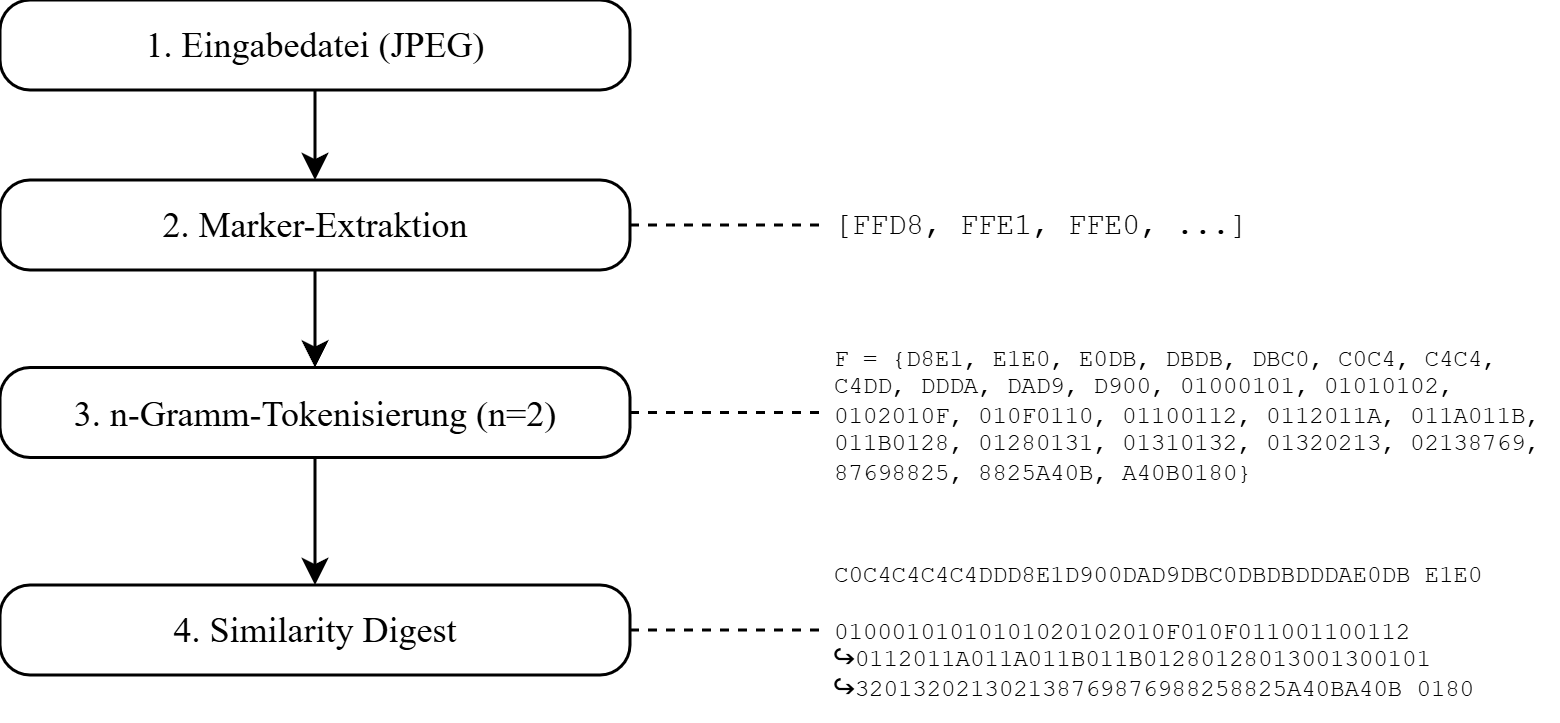
\includegraphics[width=0.9\linewidth]{grafiken/vorgehen-mssh.drawio.png}
    \caption{TODO: vorgehen-mssh.drawio.png}
    \label{fig:vorgeh-mssh}
\end{figure}

Das Konzept des $n$-Gramms stammt ursprünglich aus der Computerlinguistik und bezeichnet eine Abfolge von $n$ aufeinanderfolgenden Elementen in einer Datenreihe \cite[Kap. 3]{jurafsky_speech_2026}. Wendet man dies auf Dateistrukturen an, wandert ein festes Sichtfenster (Sliding Window) der Länge $n$ schrittweise über die extrahierten Format-Marker. So entsteht eine Menge an überlappenden Teilsequenzen. Der Vorteil dieser Methode ist, dass lokale Bausteine und ihre Reihenfolge erhalten bleiben. Dadurch lassen sich Dateien auch dann zuverlässig vergleichen, wenn sie nicht vollständig, sondern nur in bestimmten Teilbereichen strukturell übereinstimmen \cite[Kap. 3.2]{klier_media_2025}.

Die exakte Reihenfolge und das Auftauchen struktureller Elemente besitzen für die forensische Differenzierung von Quellen eine hohe Prägnanz. Bei der Übertragung dieses Prinzips auf Videodaten ergeben sich neue Herausforderungen. Wie in Abschnitt \ref{kap:aufbau_mp4} dargelegt, basiert die Architektur von MP4-Dateien nicht auf einer linearen Abfolge von Markern, sondern auf einer tief verschachtelten, objektorientierten Baumstruktur \cite[Kap. 4]{iso_14496-12_2022}.

Die grundlegende Methodik des MSSH weist mehrere Besonderheiten auf, die für die Übertragbarkeit auf MP4-Container relevant sind. Ein zentraler Vorzug liegt in der Einfachheit des Verfahrens, da Klier und Baier bewusst auf komplexe, überwachte Klassifikatoren verzichten und stattdessen einen charmant simplen Mengenabgleich mittels Similarity Digest wählen. Dadurch lässt sich für jede erdenkliche forensische Fragestellung ein eigener Source Digest bilden, unabhängig davon, ob eine Zuordnung auf Geräte, Modell oder Herstellerebene, eine Unterscheidung der Aufnahmeart oder eine Erkennung der Verarbeitungsart durch soziale Netzwerke im Vordergrund steht. Diese Flexibilität ergibt sich daraus, dass ein Source Digest lediglich aus der Mengenvereinigung mehrerer diverser Aufnahmen derselben Quelle gebildet wird, wodurch je nach gewünschter Granularität unterschiedliche Quellklassen definiert werden können, ohne das methodische Vorgehen selbst anzupassen. \cite[Kap. 3.1]{klier_media_2025}

Im Gegensatz zu überwachten Verfahren wie Entscheidungsbäumen oder Linear Discriminant Analysis entfällt zudem ein aufwändiges vorheriges Trainieren auf einem vollständigen Klassensatz, da lediglich eine kleine, diverse Teilmenge zur Digest Bildung benötigt wird, wie auch der Verfahrenssteckbrief in \cref{tab:steckbrief-klier} in der Zeile zu Test und Trainingsdaten zusammenfasst. Der anschließende Abgleich einer unbekannten Datei mit einem solchen Referenz-Digest erfolgt über einen einfachen Mengenvergleich mittels Jaccard- oder Tversky-Index, wobei Letzterer gezielt tolerant gegenüber Merkmalen ist, die nur im Source Digest, aber nicht in der Prüfdatei vorkommen, und umgekehrt strenger reagiert. \cite[Kap. 3.5]{klier_media_2025} 

In der Evaluation über sieben JPEG-Datensätze erreicht MSSH trotz dieser methodischen Schlichtheit AUC-Werte von über 0,90 auf Geräte-, Modell- und Markenebene sowie von über 0,85 bei Social-Media-Verarbeitung und erzielt damit eine mit ressourcenintensiven, PRNU-basierten Verfahren zur Source Camera Identification vergleichbare oder überlegene Erkennungsleistung, bei deutlich geringerem Berechnungsaufwand \cite[Kap. 4.4]{klier_media_2025}. Klier und Baier benennen die Übertragung dieses schlanken Konzepts auf komplexere Container-Formate wie MP4 explizit als vielversprechende Erweiterung, sofern die Strukturextraktion formatspezifisch angepasst wird \cite[Kap. 5]{klier_media_2025}.

Für das in dieser Arbeit zu entwickelnde Feature-Design (TF1) folgt daraus, dass die lineare Sequenz und die relative Reihenfolge der Boxen als wichtiges Indiz beibehalten und beim Extraktionsprozess sowie der linearen Darstellung der Struktur beachtet werden sollten.
